\chapter{Prototipo Incremental}

En el siguiente capítulo se describirá la implementación del segundo prototipo del sistema, el prototipo incremental. En este capítulo se incluirán los pasos necesarios para instalar la última versión de Erlang OTP sobre Easpberry-Pi así como versiones anteriores y se realizarán pruebas con este lenguaje para analizar su comportamiento sobre este sistema.

\section{Instalación de Erlang sobre Raspberry-Pi}
La instalación de Erlang en la placa R-Pi es sencilla y está más que probada ya que el sistema operativo Raspbian está basado en Debian. Podemos encontrar multitud de manuales de cómo hacerlo y en el caso de este proyecto se ha decidido utilizar \textit{Raspbian snap} para su instalación a través de terminal de texto.

Primero debe instalarse <<snapd>>, reiniciar la placa R-Pi e instalar core snap para obtener la última versión de snapd:
\begin{lstlisting}[style=terminal]
$ sudo apt update
$ sudo apt install snapd
$ sudo reboot
$ sudo snap install core
\end{lstlisting}

Por último, se instala Erlang/OTP mediante el siguiente comando:
\begin{lstlisting}[style=terminal]
$ sudo snap install erlang --classic
\end{lstlisting}

Tras realizar estos pasos ya disponemos de la última versión de Erlang disponible para la placa R-Pi con Raspbian, si ejecutamos el comando siguiente podemos acceder a la consola de Erlang donde veremos su versión y podremos ejecutar nuestros módulos, puede observarse su salida en el código de la Figura~\ref{fig:erlangRasp}.

\begin{lstlisting}[style=terminal]
$ erl
\end{lstlisting}

\begin{figure}[h]
\centering
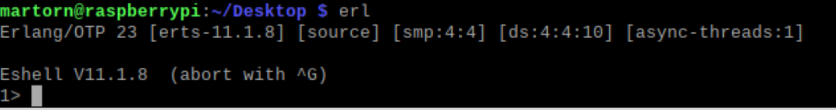
\includegraphics[scale=0.8]{images/erlangRaspberry.png}
\caption[Primer acceso a Erlang en Raspberry-Pi]{Visualización del terminal de la placa R-Pi al realizar el primer acceso a Erlang, puede visualizarse la versión del mismo.}%
\label{fig:erlangRasp}
\end{figure}


Puede darse el caso de necesitar alguna versión anterior de Erlang ya que alguna de las herramientas a utilizar no sea compatible con la última, si se desea instalar alguna versión específica de Erlang en la placa R-Pi deben de seguirse los siguientes pasos:

Primero debe actualizarse el sistema e instalar las dependencias que Erlang necesita para funcionar en este tipo de instalaciones:\\
 
\begin{lstlisting}[style=terminal]
$ sudo apt update
$ sudo apt upgrade
$ sudo apt install build-essential libncurses5-dev openssl libssl-dev fop xsltproc unixodbc-dev
\end{lstlisting}

Una vez realizado este paso debemos encontrar la versión deseada en el sitio Web oficial de descargas de Erlang \cite{erlang.orgStart}, es importante elegir correctamente una versión que sea compatible con la arquitectura de la placa R-Pi como puede ser armhf o arm64.

Tras la elección de la versión procedemos a descargarla y descomprimirla ya sea desde la página o desde terminal ejecutando los siguientes comandos:\\

\begin{lstlisting}[style=terminal]
$ wget https://erlang.org/download/otp_src_24.0.tar.gz
$ tar -xf otp_src_24.0.tar.gz
\end{lstlisting}

Por último, debemos acceder al directorio en el que se ha descomprimido el archivo y realizar la instalación de la siguiente manera:\\

\begin{lstlisting}[style=terminal]
$ cd otp_src_24.0
$ ./configure
$ make
$ sudo make install
\end{lstlisting}

Siguiendo los pasos anteriores podemos realizar en la placa R-Pi cualquier instalación de alguna versión Erlang que sea compatible con la misma.

\section{Pruebas con Erlang}

Para finalizar con este capítulo se ha creado un programa en Erlang para poner a prueba el rendimiento de este lenguaje sobre la placa R-Pi y su correcto funcionamiento, a su vez se ha creado un programa en Python con igual funcionalidad. El programa realiza una operación muy sencilla, calcula la suma de los primeros N números naturales y muestra el resultado, por último, para valorar el tiempo que tarda en realizar esta operación se muestra el tiempo de ejecución del programa en microsegundos. 

En el siguiente listado (tiempoEjecucion.erl) se muestra el código Erlang creado y la salida de tiempo obtenida realizando operaciones con $N$ números diferentes (Figura~\ref{fig:pruebaErlang} con $N=100$ y Figura~\ref{fig:pruebaErlang100000} con $N=100000$).\\

\lstset{language=Erlang, breaklines=true, basicstyle=\sffamily\footnotesize}
\begin{lstlisting}[frame=single, caption=tiempoEjecucion.erl]

-module(tiempoEjecucion).
-export([sum/1]).

sum(N) ->
    Start = os:timestamp(),
    Result = lists:sum(lists:seq(1, N)),
    End = os:timestamp(),
    Time = timer:now_diff(End, Start),
    io:format("La suma es ~p~n", [Result]),
    io:format("Tiempo de ejecucion: ~p microsegundos~n", [Time]).
\end{lstlisting}

\begin{figure}[h]
\centering
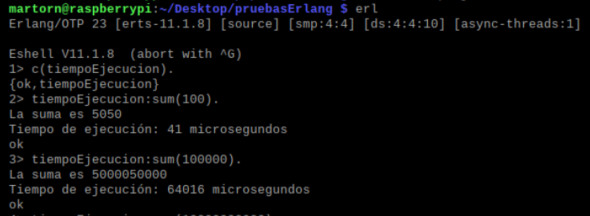
\includegraphics[scale=1.3]{images/pruebaErlang.png}
\caption[Salida de terminal suma de N=100 con Erlang]{Visualización de la salida de terminal de la placa R-Pi al ejecutar el programa que hace la suma de N en Erlang con N=100.}%
\label{fig:pruebaErlang}
\end{figure}

\begin{figure}[h]
\centering
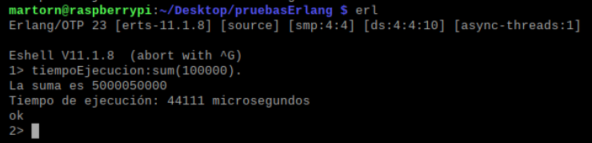
\includegraphics[scale=1.3]{images/pruebaErlang100000.png}
\caption[Salida de terminal suma de N=100000 con Erlang]{Visualización de la salida de terminal de la placa R-Pi al ejecutar el programa que hace la suma de N en Erlang con N=100000.}%
\label{fig:pruebaErlang100000}
\end{figure}

\clearpage
El siguiente código Python (tiempoEjecucion.py) tiene la misma funcionalidad que el código Erlang anterior, en la Figura~\ref{fig:pruebaPython} y Figura~\ref{fig:pruebaPython100000} pueden observarse las salidas obtenidas por el programa con los valores 100 y 100000 de N respectivamente.


\lstset{language=Python, breaklines=true, basicstyle=\footnotesize}
\begin{lstlisting}[frame=single, caption=tiempoEjecucion.py]
import time

def sum_numbers(n):
    start = time.time()
    result = sum(range(1, n+1))
    end = time.time()
    elapsed_time = (end - start) * 1000000
    print(f "La suma es {result}")
    print(f "Tiempo de ejecucion: {elapsed_time:.2f} microsegundos")

n = int(input("Ingrese el valor de N: "))
sum_numbers(n)
\end{lstlisting}

\begin{figure}[h]
\centering
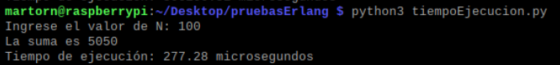
\includegraphics[scale=1.3]{images/pruebaPython100.png}
\caption[Salida de terminal suma de N=100 con Python]{Visualización de la salida de terminal de la placa R-Pi al ejecutar el programa que hace la suma de N en Python con N=100.}%
\label{fig:pruebaPython}
\end{figure}

\begin{figure}[h]
\centering
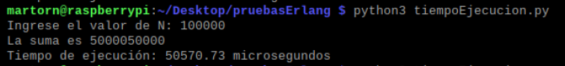
\includegraphics[scale=1.3]{images/pruebaPython.png}
\caption[Salida de terminal suma de N=100000 con Erlang]{Visualización de la salida de terminal de la placa R-Pi al ejecutar el programa que hace la suma de N en Python con N=100000.}%
\label{fig:pruebaPython100000}
\end{figure}

Los resultados se muestran en la tabla del Cuadro~\ref{tab:tiempos1}. Puede verse que el programa creado en Erlang es algo más rápido que el programado en Python pero es una diferencia muy poco significativa. Por otro lado, el código C es algo más rápido que ambos. De cualquier manera, vemos que Erlang parece plenamente funcional en la placa R-Pi y que su rendimiento es similar al de Python, lenguaje mucho más frecuente en este tipo de dispositivos. Para obtener conclusiones más precisas sobre las velocidades de cada lenguaje sería conveniente realizar muchas más pruebas o ejecuciones con diferentes repeticiones. 

\begin{table}[h]
\begin{center}
\sffamily
\begin{tabular}{lcc}
\toprule[1,7pt]
%\begin{tabular}{|>{\columncolor{gray!20}}lcc|}\hline
     &  \multicolumn{2}{c}{Tiempo invertido (µs).} \\
     \cline{2-3}
%\rowcolor{gray!20}
Lenguaje & 100 repeticiones & 100,000 repeticiones \\
\midrule[1.2pt]
Erlang & 41 & 44111 \\
\hline
Python & 277 & 50570 \\
\hline
C & 28 & 39587 \\
\bottomrule[1,7pt]
\end{tabular}
\caption[Comparativa de tiempos de ejecución]{Comparativa de tiempos de ejecución entre Erlang, Python y C medido en microsegundos realizando 100 y 100000 repeticiones.}%
\label{tab:tiempos1}
\end{center}
\end{table}







 